\documentclass{beamer}
\usecolortheme{seahorse}
\useinnertheme{rectangles}
\useoutertheme{infolines}
\usepackage{tikz}
\usetikzlibrary{positioning}
\usepackage{soul}


\title[ngUML 2023 Q4]{
    ngUML End of Year
}
\subtitle{
    Towards an OSS framework for AI-assisted MDE
}
\author{Max Boone}
\institute{LIACS}
\date{25th of May 2023}

\begin{document}

\frame{\titlepage}

\begin{frame}
    \frametitle{Contents}
    \tableofcontents
\end{frame}

\section{Looking Back}

\subsection{Refactoring}

\begin{frame}{Refactoring}{Front-End}
    \begin{columns}
        \column{0.75\linewidth}
            \begin{itemize}
                \item Dependencies (Carbon, Palantir, MUI)
                \item Multiple Diagrams (Projects \& Systems)
                \item Floating (Editor) Panes
                \item Diagram Editor
            \end{itemize}
        \column{0.25\linewidth}
            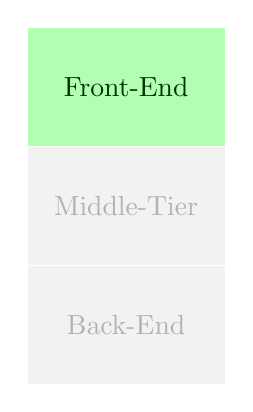
\begin{tikzpicture}[
                    active/.style={fill=green!30, text=black!80!green, minimum width=2.5cm, minimum height=1.5cm},
                    inactive/.style={fill=gray!10, text=gray!60, minimum width=2.5cm, minimum height=1.5cm},
                ]
                %Nodes
                \node[active]   (fe)                 {Front-End};
                \node[inactive] (mt) [below=0 of fe] {Middle-Tier};
                \node[inactive] (be) [below=0 of mt] {Back-End};
            \end{tikzpicture}
    \end{columns}
\end{frame}

\begin{frame}{Refactoring}{Front-End}
    \begin{columns}
        \column{0.75\linewidth}
            \begin{itemize}
                \item Dependencies (Carbon, Palantir, MUI)
                \item Multiple Diagrams (Projects \& Systems)
                \item Diagram Editor
            \end{itemize}
        \column{0.25\linewidth}
            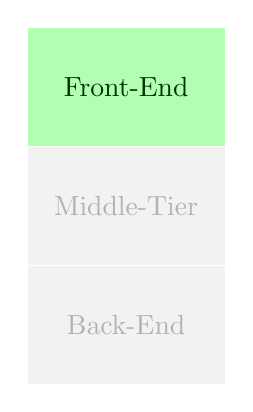
\begin{tikzpicture}[
                    active/.style={fill=green!30, text=black!80!green, minimum width=2.5cm, minimum height=1.5cm},
                    inactive/.style={fill=gray!10, text=gray!60, minimum width=2.5cm, minimum height=1.5cm},
                ]
                %Nodes
                \node[active]   (fe)                 {Front-End};
                \node[inactive] (mt) [below=0 of fe] {Middle-Tier};
                \node[inactive] (be) [below=0 of mt] {Back-End};
            \end{tikzpicture}
    \end{columns}
\end{frame}

\end{document}